%% ID: foggy_jet
%% TITLE: A Jet in the Fog
%% TYPE: question
%% QUESTIONTYPE: numerical
%% CONCEPTS: eq_of_motions_diff
%% VIDEOS: 
%% LEVEL: 3
%% TOPIC: mechanics/kinematics
%% ORDER: 6

\begin{problem}[Jan_Foggy_Day] 
{\exposition{A person is standing on top of a mountain on a foggy day. The fog obscures their vision beyond a distance \valuedef{r}{500}{m}. A fighter jet is travelling in a straight line on a horizontal flight path at the same altitude as the person on the mountain. The person uses a stopwatch to measure the time between when the jet first becomes visible and when the jet is loudest to them. They then measures the time between the loudest noise they hear and the jet exiting their field of vision. Their first measurement is \valuedef{T\s{1}}{1.6}{s}, and their second is \valuedef{T\s{1}}{1.0}{s}}
\\ \\
\item \question[a]{Find the distance, \vari{d} to the point of closest approach.}
\item \question[b]{ind the velocity, \vari{V} of the jet.} 
\hinta{Take the speed of sound to be \valuedef{V\s{s}}{340}{m s\sup{-1}}, and assume that the loudest sound wave is emitted when the jet is at its closest point to the person. Neglect delays due to the speed of light having finite speed.}}
{\textit{Written by JZ and JS for The Rutherford Schools Physics Project.}}
{This question is all about where the jet actually is compared to where it was when the person hears it at its closest point, as sound only travels at \valuedef{V\s{s}}{340}{m s\sup{-1}}.

\begin{figure}[h]
	\centering
	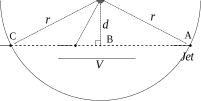
\includegraphics[width=0.5\textwidth]{Kinematics_Jan_Foggy_Day}
	\caption{}
	\label{fig:Kinematics_Jan_Foggy_Day}
\end{figure}

We should briefly interpret Figure \ref{fig:Kinematics_Jan_Foggy_Day}. The jet first enters the person's field of vision at A and travels at speed \vari{V} to C, passing through the closest point of approach, B during its flight. An obvious (but useful) point to note is that AB = BC.

\begin{figure}[h]
	\centering
	\includegraphics[width=0.5\textwidth]{Kinematics_Jan_Foggy_Day_2}
	\caption{}
	\label{fig:Kinematics_Jan_Foggy_Day_2}
\end{figure}


Next, look at Figure \ref{fig:Kinematics_Jan_Foggy_Day_2}. $\Delta T$ is the time taken for the sound to reach the observer. \vari{T\s{1}}, as recorded by the person, is how long the jet has taken to travel $[\textrm{AB} + (\Delta T \times V)]$m, and \vari{T\s{2}} is the time taken for the remaining distance.

\begin{align*} \Delta T = T\s{1} - \frac{T\s{1}+T\s{2}}{2} = \frac{T\s{1}-T\s{2}}{2} \end{align*}

Also, since \vari{\Delta T} is the time taken for the sound to reach the observer: \begin{align*} d = V\s{s}\Delta{T}\end{align*}

Hence \begin{align*} d = V\s{s}\left[\frac{T\s{1}-T\s{2}}{2}\right]\end{align*}

\answer[a]{\valuedef{d}{100}{m} to 2 significant figures}

We have a right-angled triangle ABO, so can use Pythagoras' Theorem to form an equation for distance, and then solve for $V$:

\begin{align*} &(AB)^{2} + (OB)^{2} = (OA)^{2} \\
\\&\left[V(T\s{1} - \Delta{T})\right]^{2} + d^{2} = r^{2} \\
\\&\left[V\left(T\s{1} - \frac{d}{V\s{s}}\right)\right]^{2} + d^{2} = r^{2} \\ 
\\&\left[V\left(T\s{1} - \frac{V\s{s}}{V\s{s}}\left[\frac{T\s{1} - T\s{2}}{2}\right]\right)\right]^{2} + V\s{s}^{2}\left[\frac{T\s{1} - T\s{2}}{2}\right]^{2} = r^{2} \\
\\&V^{2}\left(T\s{1} - \left[\frac{T\s{1}-T\s{2}}{2}\right]\right)^{2} + V\s{s}^{2}\left[\frac{T\s{1} - T\s{2}}{2}\right]^{2} = r^{2} \\
\\&V = \sqrt{\frac{r^{2} - V\s{s}^{2}\left(\frac{T\s{1}-T\s{2}}{2}\right)^{2}}{T\s{1} - \frac{T\s{1}-T\s{2}}{2}}}\\
\\&V = \frac{2\sqrt{r^{2} - \left(\frac{V\s{s}}{2}\right)^{2}(T\s{1}-T\s{2})^{2}}}{(T\s{1}+T\s{2})}\end{align*}

Putting in numbers:

\begin{align*} V &= \frac{2\sqrt{(500)^{2} - \left(\frac{340}{2}\right)^{2}(1.6 - 1.0)^{2}}}{(1.6+1.0)} \textrm{ ms}^{-1}\\
\\ &= \frac{2\sqrt{239596}}{2.6} \textrm{ ms}^{-1}\\
\\ &= \frac{979.0}{2.6} \textrm{ ms}^{-1}
\\ &= 376.5 \textrm{ ms}^{-1} \end{align*}
which is about Mach 1.1 (or 1.1 times the speed of sound, $V\s{s}$) which is roughly the cruising speed of a modern fighter jet!

\answer[b]{\valuedef{V}{380}{m s\sup{-1}} to 2 significant figures.}


}
\end{hint}